\documentclass[conference]{IEEEtran}
\IEEEoverridecommandlockouts

\usepackage{cite}
\usepackage{amsmath,amssymb,amsfonts}
\usepackage{algorithmic}
\usepackage{graphicx}
\usepackage{textcomp}
\usepackage{xcolor}
\usepackage{booktabs}
\usepackage{multirow}
\usepackage{url}
\usepackage{microtype}
\usepackage{xspace}
% Auto-generated by python/make_paper_tables.py - DO NOT EDIT MANUALLY

% Single source of truth for all quantitative figures in paper

\newcommand{\valNtenAcc}{90.17\xspace}
\newcommand{\valNtenAccPct}{90.17\%\xspace}
\newcommand{\valNtenAccCILow}{82.7}
\newcommand{\valNtenAccCIHigh}{95.9}
\newcommand{\valNtenBalAcc}{90.53\xspace}
\newcommand{\valNtenBalAccPct}{90.53\%\xspace}
\newcommand{\valNtenFOne}{90.49\xspace}
\newcommand{\valNtenFOnePct}{90.49\%\xspace}
\newcommand{\valNtenFOneCILow}{81.9}
\newcommand{\valNtenFOneCIHigh}{96.2}
\newcommand{\valNtenSens}{86.25\xspace}
\newcommand{\valNtenSensPct}{86.25\%\xspace}
\newcommand{\valNtenSpec}{94.81\xspace}
\newcommand{\valNtenSpecPct}{94.81\%\xspace}
\newcommand{\valNtenRocAuc}{0.9361\xspace}
\newcommand{\valNfiveAcc}{85.42\xspace}
\newcommand{\valNfiveAccPct}{85.42\%\xspace}
\newcommand{\valNfiveAccCILow}{76.5}
\newcommand{\valNfiveAccCIHigh}{93.3}
\newcommand{\valNfiveBalAcc}{86.10\xspace}
\newcommand{\valNfiveFOne}{85.32\xspace}
\newcommand{\valNfiveSens}{78.12\xspace}
\newcommand{\valNfiveSpec}{94.07\xspace}
\newcommand{\valNoneAcc}{84.07\xspace}
\newcommand{\valNoneAccCILow}{75.2}
\newcommand{\valNoneAccCIHigh}{92.0}
\newcommand{\valNoneBalAcc}{84.56\xspace}
\newcommand{\valNoneFOne}{84.28\xspace}
\newcommand{\valNoneSens}{78.75\xspace}
\newcommand{\valNoneSpec}{90.37\xspace}
\newcommand{\valNtwoAcc}{83.39\xspace}
\newcommand{\valNtwoAccCILow}{73.8}
\newcommand{\valNtwoAccCIHigh}{91.8}
\newcommand{\valNthreeAcc}{82.37\xspace}
\newcommand{\valNthreeAccCILow}{73.0}
\newcommand{\valNthreeAccCIHigh}{91.0}
\newcommand{\valControlNoCalibAcc}{78.64\xspace}
\newcommand{\valControlNoCalibAccPct}{78.64\%\xspace}
\newcommand{\valControlNoCalibAccCILow}{69.0}
\newcommand{\valControlNoCalibAccCIHigh}{88.0}
\newcommand{\valControlNoCalibBalAcc}{79.50\xspace}
\newcommand{\valControlNoCalibSens}{69.38\xspace}
\newcommand{\valControlNoCalibSpec}{89.63\xspace}
\newcommand{\valControlLeakyTwoNineFiveAcc}{89.83\xspace}
\newcommand{\valControlLeakyTwoNineFiveAccPct}{89.83\%\xspace}
\newcommand{\valControlLeakyTwoNineFiveAccCILow}{81.1}
\newcommand{\valControlLeakyTwoNineFiveAccCIHigh}{96.7}
\newcommand{\valControlLeakyTwoNineFiveBalAcc}{90.51\xspace}
\newcommand{\valLegacyFourFourFiveAcc}{92.13\xspace}
\newcommand{\valLegacyFourFourFiveAccPct}{92.13\%\xspace}
\newcommand{\valLegacyFourFourFiveAccCI}{[86.4, 97.1]}
\newcommand{\valLegacyFourFourFiveBalAcc}{90.02\xspace}
\newcommand{\valLegacyFourFourFiveFOne}{88.29\xspace}
\newcommand{\valLegacyFourFourFiveSens}{82.50\xspace}
\newcommand{\valLegacyFourFourFiveSpec}{97.54\xspace}
\newcommand{\valPairedGainNten}{+11.53\xspace}
\newcommand{\valPairedGainNtenCILow}{+5.07}
\newcommand{\valPairedGainNtenCIHigh}{+18.06}
\newcommand{\valPairedGainNfive}{+6.78\xspace}
\newcommand{\valPairedGainNfiveCILow}{+0.68}
\newcommand{\valPairedGainNfiveCIHigh}{+13.22}
\newcommand{\valPairedGainNthree}{+3.73\xspace}
\newcommand{\valPairedGainNthreeCILow}{$-$4.05}
\newcommand{\valPairedGainNthreeCIHigh}{+11.56}
\newcommand{\valPairedGainNtwo}{+4.75\xspace}
\newcommand{\valPairedGainNtwoCILow}{$-$3.06}
\newcommand{\valPairedGainNtwoCIHigh}{+12.72}
\newcommand{\valPairedGainNone}{+5.42\xspace}
\newcommand{\valPairedGainNoneCILow}{$-$2.70}
\newcommand{\valPairedGainNoneCIHigh}{+13.40}
\newcommand{\valPairedGainNtenVsNfive}{+4.75\xspace}
\newcommand{\valPairedGainNtenVsNfiveCILow}{+0.68}
\newcommand{\valPairedGainNtenVsNfiveCIHigh}{+9.52}
\newcommand{\valPairedGainNtenVsLeaky}{+0.34\xspace}
\newcommand{\valPairedGainNtenVsLeakyCILow}{$-$3.36}
\newcommand{\valPairedGainNtenVsLeakyCIHigh}{+4.79}
\newcommand{\valAblFourRawAcc}{75.25\xspace}
\newcommand{\valAblFourNtenAcc}{88.81\xspace}
\newcommand{\valAblEightRawAcc}{78.64\xspace}
\newcommand{\valAblEightNtenAcc}{90.17\xspace}
\newcommand{\valAblThirteenRawAcc}{78.31\xspace}
\newcommand{\valAblThirteenNtenAcc}{89.49\xspace}
\newcommand{\valTauThirtyFiveAcc}{87.80\xspace}
\newcommand{\valTauThirtyFiveAccPct}{87.80\%\xspace}
\newcommand{\valTauThirtyFiveSens}{88.75\xspace}
\newcommand{\valTauThirtyFiveSensPct}{88.75\%\xspace}
\newcommand{\valTauThirtyFiveSpec}{86.67\xspace}
\newcommand{\valTauThirtyFiveSpecPct}{86.67\%\xspace}
\newcommand{\valTauThirtyFiveBalAcc}{87.71\xspace}
\newcommand{\valTauThirtyFiveFOne}{88.75\xspace}
\newcommand{\valLegacyTauThirtyFiveAcc}{92.36\xspace}
\newcommand{\valLegacyTauThirtyFiveAccPct}{92.36\%\xspace}
\newcommand{\valLegacyTauThirtyFiveSens}{86.25\xspace}
\newcommand{\valLegacyTauThirtyFiveSensPct}{86.25\%\xspace}
\newcommand{\valLegacyTauThirtyFiveSpec}{95.79\xspace}
\newcommand{\valLegacyTauThirtyFiveSpecPct}{95.79\%\xspace}
\newcommand{\valSvmAcc}{90.17\xspace}
\newcommand{\valSvmAccPct}{90.17\%\xspace}
\newcommand{\valSvmSens}{84.38\xspace}
\newcommand{\valSvmSensPct}{84.38\%\xspace}
\newcommand{\valSvmSpec}{97.04\xspace}
\newcommand{\valSvmSpecPct}{97.04\%\xspace}
\newcommand{\valOtherModelAccMin}{86.10\xspace}
\newcommand{\valOtherModelAccMax}{88.14\xspace}
\newcommand{\valNumSubjects}{15\xspace}
\newcommand{\valTotalWindows}{445\xspace}
\newcommand{\valBaselineWindows}{285\xspace}
\newcommand{\valStressWindows}{160\xspace}
\newcommand{\valEvalWindows}{295\xspace}
\newcommand{\valEvalBaselineWindows}{135\xspace}
\newcommand{\valEvalStressWindows}{160\xspace}
\newcommand{\valMajorityClassPct}{54.24\%\xspace}
\newcommand{\valSamplingRateHz}{700\xspace}
\newcommand{\valWindowDurationSec}{60\xspace}
\newcommand{\valBiquadMeanCycles}{251\xspace}
\newcommand{\valBiquadMinCycles}{249\xspace}
\newcommand{\valBiquadMaxCycles}{281\xspace}
\newcommand{\valBiquadMinUs}{1.464\xspace}
\newcommand{\valBiquadMeanUs}{1.476\xspace}
\newcommand{\valBiquadMaxUs}{1.652\xspace}
\newcommand{\valBiquadCpuLoad}{0.0517\%\xspace}
\newcommand{\valDwtTrialCount}{1,000\xspace}
\newcommand{\valUartBaudRate}{115,200\xspace}
\newcommand{\valFlashSampleCount}{2,100\xspace}
\newcommand{\valFlashSamples}{\valFlashSampleCount}
\newcommand{\valFlashSampleSec}{6\xspace}
\newcommand{\valLyapunovPrimaryLOne}{+0.4199\xspace}
\newcommand{\valLyapunovPrimaryLTwo}{+0.2639\xspace}
\newcommand{\valLyapunovPrimaryDKY}{3.0241\xspace}
\newcommand{\valLyapunovRangeLOneLow}{+0.4182\xspace}
\newcommand{\valLyapunovRangeLOneHigh}{+0.5282\xspace}
\newcommand{\valLyapunovRangeLTwoLow}{+0.2361\xspace}
\newcommand{\valLyapunovRangeLTwoHigh}{+0.2995\xspace}
\newcommand{\valSubjImproveCount}{9\xspace}
\newcommand{\valSubjUnchangedCount}{4\xspace}
\newcommand{\valSubjDecreaseCount}{2\xspace}
\newcommand{\valSubjTotalCount}{15\xspace}
\newcommand{\valHilPackets}{10,000\xspace}
\newcommand{\valHilWireBytes}{200,000\xspace}
\newcommand{\valHilPayloadBytes}{80,000\xspace}
\newcommand{\valWireEntropy}{7.9977\xspace}
\newcommand{\valFullFrameEntropy}{7.0705\xspace}
\newcommand{\valChiSquareStat}{257.79\xspace}
\newcommand{\valChiSquareP}{0.4394\xspace}
\newcommand{\valDivergence}{-27.64\xspace}


\def\BibTeX{{\rm B\kern-.05em{\sc i\kern-.025em b}\kern-.08em
    T\kern-.1667em\lower.7ex\hbox{E}\kern-.125emX}}

\begin{document}

\title{How Much Labelled Rest is Needed? Leak-Free Baseline Calibration for Single-Lead ECG Stress Detection on WESAD}

\author{\IEEEauthorblockN{Mukesh Yadav}
\IEEEauthorblockA{\textit{Department of Electronics and Communication Engineering (ECE)} \\
\textit{JSS Academy of Technical Education}\\
Noida, Uttar Pradesh, India \\
mkpy06@gmail.com}
}

\maketitle

\begin{abstract}
Wearable ECG stress detectors often normalise a person's features against resting baseline data, but published protocols rarely say how much labelled rest is used or whether those baseline windows are also scored. We study this on the \valNumSubjects-subject WESAD chest ECG (RespiBAN, \valSamplingRateHz~Hz) with eight HRV features from \valWindowDurationSec~s windows, Logistic Regression (the model used in our original analysis) and 15-fold leave-one-subject-out validation. Features are normalised against the first $N$ resting windows ($N = 1, 2, 3, 5, 10$), which are excluded from scoring; all settings are scored on the same \valEvalWindows windows (majority-class accuracy \valMajorityClassPct). Accuracy is \valControlNoCalibAccPct without calibration, \valNfiveAccPct with $N = 5$ and \valNtenAccPct with $N = 10$. Subject-level paired bootstrap intervals for the gain over no calibration exclude zero for $N = 5$ (\valPairedGainNfive~pp [95\% CI: \valPairedGainNfiveCILow, \valPairedGainNfiveCIHigh]) and $N = 10$ (\valPairedGainNten~pp [95\% CI: \valPairedGainNtenCILow, \valPairedGainNtenCIHigh]) and include zero for $N \le 3$. The choice of $N = 10$, the feature set and the decision threshold were made after seeing results on these subjects, and intervals are unadjusted. An earlier all-baseline anchor scores \valControlLeakyTwoNineFiveAccPct on the same windows, with no detectable difference (\valPairedGainNtenVsLeaky~pp [95\% CI: \valPairedGainNtenVsLeakyCILow, \valPairedGainNtenVsLeakyCIHigh]). Separately, a 5-stage biquad IIR filter runs in \valBiquadMeanCycles cycles on an STM32G474RE, and a 20-byte telemetry frame with a hyperchaotic keystream obfuscation layer was replayed over UART for \valHilPackets packets with no CRC errors; this obfuscation is not cryptographic protection.
\end{abstract}

\begin{IEEEkeywords}
Electrocardiogram (ECG), Heart Rate Variability (HRV), Acute Stress Detection, WESAD, Leave-One-Subject-Out (LOSO), Baseline Calibration, Edge Computing, ARM Cortex-M4, STM32.
\end{IEEEkeywords}

\section{Introduction}
Psychological stress activates the sympathetic-adreno-medullary (SAM) and hypothalamic-pituitary-adrenal (HPA) axes, inducing autonomic nervous system (ANS) shifts characterized by sympathetic activation and parasympathetic (vagal) withdrawal \cite{kirschbaum1993trier, kim2018stress}. Continuous monitoring via wearable electrocardiography (ECG) offers a direct, non-invasive window into cardiac autonomic regulation through heart rate variability (HRV) analysis \cite{taskforce1996hrv, shaffer2017overview}. Wearable stress detection has been studied in driving and daily-life settings \cite{healey2005detecting, can2019continuous}.

Despite significant advances in affective computing, translating laboratory ECG models to wearable devices raises two practical issues:
\begin{enumerate}
    \item \textit{Baseline Heterogeneity and Data Leakage:} Resting HRV differs across individuals \cite{shaffer2017overview}, so features are often normalised per person. Evaluating with record-wise splits can overestimate accuracy for new users \cite{saeb2017need}; WESAD \cite{schmidt2018wesad} supports leave-one-subject-out evaluation. Stress inference from wearable ECG and respiration has been reported in laboratory and field data \cite{plarre2011continuous}.
    \item \textit{Telemetry Privacy:} Streaming raw physiological signals over wireless links can expose personal data \cite{jiang2023wban}. This paper tests only a lightweight obfuscation layer on a microcontroller, not cryptographic protection.
\end{enumerate}

To address these challenges, this study provides three contributions:
\begin{enumerate}
    \item We evaluate the impact of baseline calibration length ($N \in \{1, 2, 3, 5, 10\}$ initial resting windows, excluded from scoring) on single-channel chest ECG stress detection under 15-fold LOSO-CV on \valEvalWindows common evaluation windows, showing a paired accuracy gain whose interval excludes zero of \valPairedGainNten~pp at $N=10$ and \valPairedGainNfive~pp at $N=5$, whereas calibrations at $N \le 3$ yield intervals spanning zero.
    \item A leak-free ablation across 1, 4, 8, and 13 HRV features showing that eight core time, frequency, and nonlinear metrics achieve \valNtenAccPct accuracy, with 13 features showing no improvement (\valAblThirteenNtenAcc\%).
    \item A measured 5-stage biquad filter cost on an STM32G474RE (\valBiquadMeanCycles mean cycles per sample) and a \valHilPackets-packet HIL replay of flash-stored ECG with an obfuscation layer.
\end{enumerate}

\section{Signal Processing and Leak-Free Methodology}

\subsection{Benchmark Dataset and Study Cohort}
We utilize the public Wearable Stress and Affect Detection (WESAD) benchmark \cite{schmidt2018wesad}, consisting of physiological recordings from \valNumSubjects healthy volunteers (mean age $27.5 \pm 2.4$ years) subjected to a verified Trier Social Stress Test (TSST) \cite{kirschbaum1993trier}. Electrocardiographic signals were acquired using a chest-worn RespiBAN device recording single-channel chest ECG at \valSamplingRateHz~Hz. Only the baseline and stress conditions are used; amusement and meditation are excluded, giving a binary task. Continuous ECG is partitioned into complete, non-overlapping \valWindowDurationSec-second windows, yielding \valBaselineWindows resting baseline windows (Class 0) and \valStressWindows acute stress windows (Class 1), totaling \valTotalWindows diagnostic windows across the cohort.

\subsection{Leak-Free Baseline Calibration Protocol}
To isolate physiological stress reactivity from resting autonomic tone without data leakage, each feature $f_{s,i}$ of subject $s$ in window $i$ undergoes subject-specific baseline relative transformation matching our open-source implementation:
\begin{equation}
    \Delta f_{s,i} = \frac{f_{s,i} - B_{s,f}}{\max(|B_{s,f}|, \epsilon)}
    \label{eq:norm}
\end{equation}
where $B_{s,f} = \frac{1}{N} \sum_{k=1}^N f_{s,k}$ is the arithmetic mean of feature $f$ computed across the first $N$ chronological baseline windows of subject $s$ ($k \in \{1, \dots, N\}$), and $\epsilon = 10^{-6}$ provides numerical stabilization against near-zero denominators. Each window is \valWindowDurationSec~s, so $N$ windows equal $N$ minutes of rest. Crucially, in each cross-validation fold, training subjects' first $N$ baseline windows are excluded from model training ($i > N$), and test subjects' first $N$ windows are excluded from test evaluation scoring. To make all $N$ comparable, the first 10 baseline windows of every subject are excluded from scoring for every $N$, so each setting is scored on the same \valEvalWindows\ windows (baseline windows 11--20 and all stress windows; majority-class baseline accuracy is \valMajorityClassPct).

In our original analysis, $B_s$ was the arithmetic mean of that subject's baseline windows (up to 20) and all \valTotalWindows windows were scored, including the baseline windows used to compute $B_s$. This leaks test baseline windows into the anchor. This leaky configuration is retained as a historical reference for the original protocol. For comparison, uncalibrated Control (a) evaluates raw feature vectors $f_{s,i}$ passed directly into fold-level standardization without subject-specific baseline subtraction or scaling, while Control (b) evaluates the leaky anchor (arithmetic mean across all available baseline windows) scored strictly on the identical \valEvalWindows common evaluation windows.

\subsection{QRS Detection and Artifact Filtering}
Raw ECG signals are conditioned offline via a zero-phase 4th-order Butterworth bandpass filter (0.5--40~Hz, $F_s = \valSamplingRateHz$~Hz) applied via forward-backward filtering (\texttt{filtfilt}) \cite{oppenheim1999discrete} to attenuate baseline wander and high-frequency noise. Ventricular depolarization QRS complexes are detected using a Pan--Tompkins-style peak-prominence detector \cite{pantompkins1985, elgendi2013fast}: rather than squaring and moving-window integration, it performs peak picking on the bandpass-filtered signal with adaptive prominence ($3.0 \times 1.4826 \times \text{MAD}$) and a refractory period distance constraint ($\ge 350$~ms). Consecutive normal-to-normal ($RR$) intervals are subjected to physiological interval gating: intervals outside $[300, 1500]$~ms ($40\text{--}200$~BPM) are rejected, as depicted in Fig.~\ref{fig:ecg_processing}.

\begin{figure}[t]
    \centering
    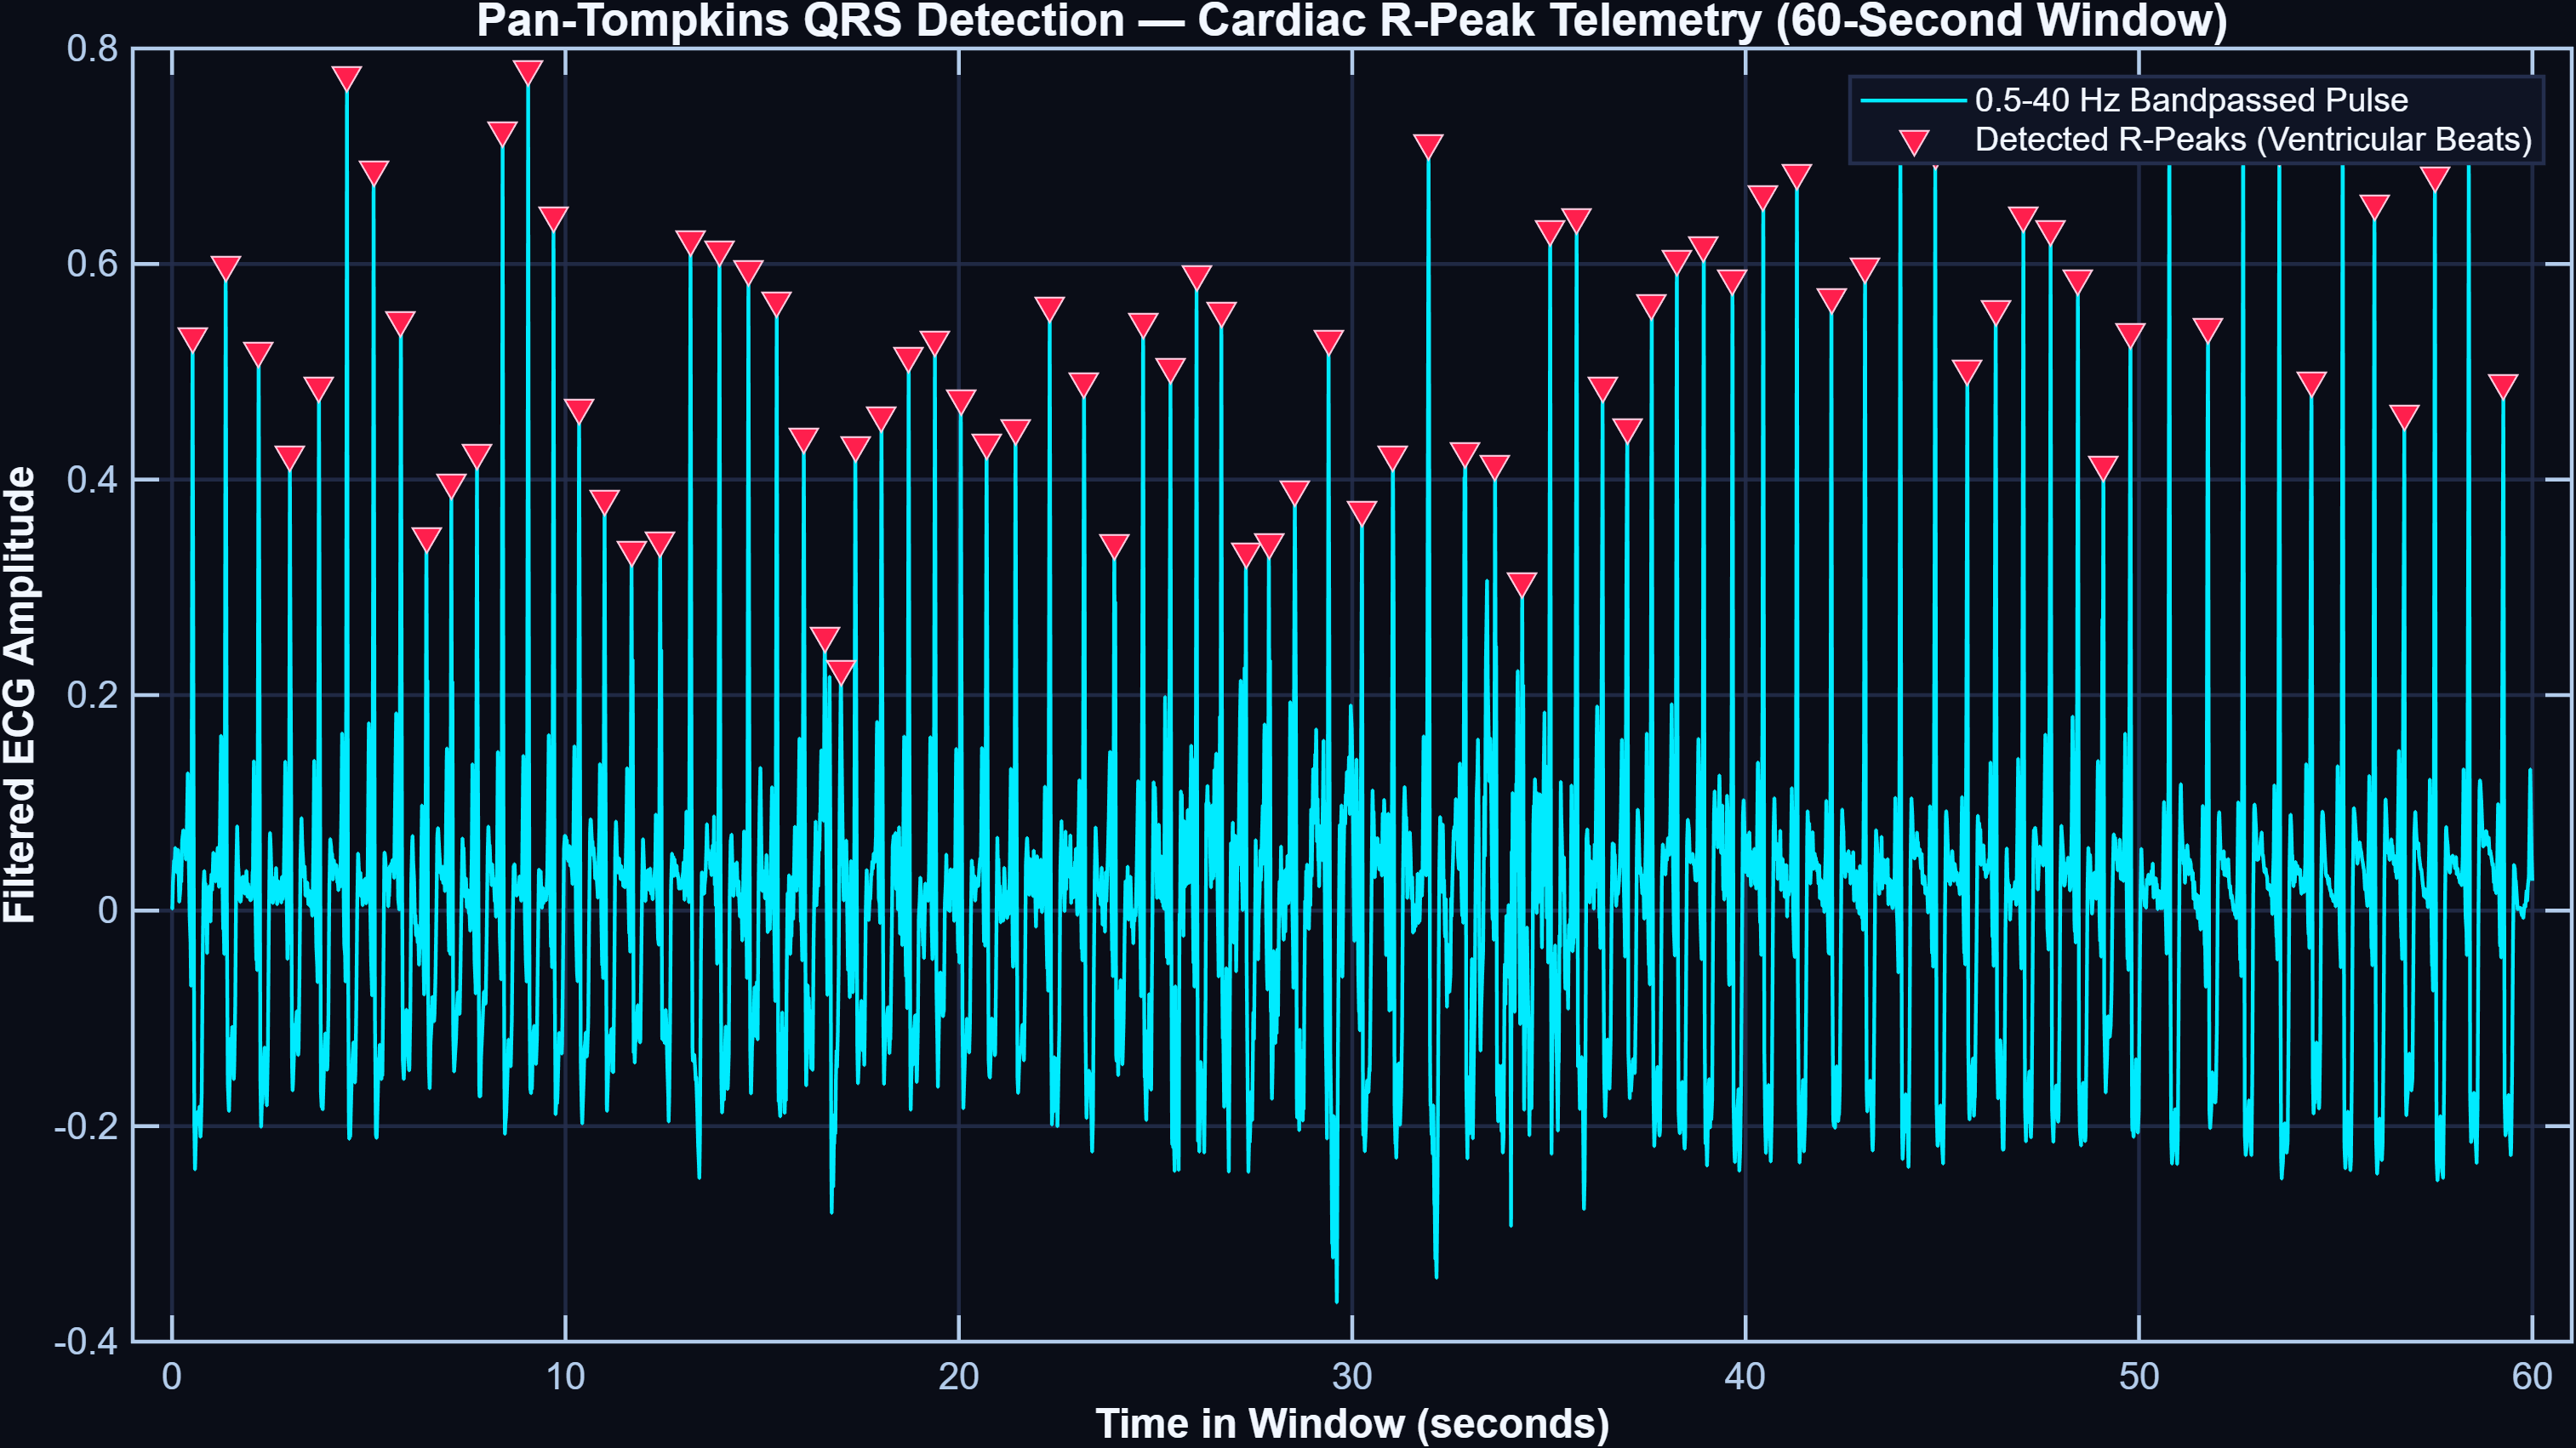
\includegraphics[width=\linewidth]{figures/DEMO_Pan_Tompkins_QRS_Detection.png}
    \caption{R-peak detection (Pan--Tompkins-style) on a \valWindowDurationSec-second window of single-channel chest ECG (RespiBAN, \valSamplingRateHz~Hz), displaying the 0.5--40~Hz bandpass-filtered waveform and detected ventricular fiducial peaks.}
    \label{fig:ecg_processing}
\end{figure}

\subsection{HRV Feature Extraction}
From artifact-filtered $RR$ sequences, eight core autonomic features are computed across time, frequency, and nonlinear domains: Mean Heart Rate (MeanHR), standard deviation of $NN$ intervals (SDNN), root mean square of successive differences (RMSSD), proportion of successive intervals differing by $>50$~ms (pNN50), Low-Frequency spectral power (LF: 0.04--0.15~Hz), High-Frequency spectral power (HF: 0.15--0.40~Hz), LF/HF ratio, and Sample Entropy ($\text{SampEn}$, $m=2, r=0.2\sigma$).

\section{Experimental Results and ML Benchmark}

\subsection{15-Fold LOSO-CV Evaluation and Model Comparison}
Table~\ref{tab:ml_benchmark} presents the performance of six machine learning architectures under 15-fold LOSO-CV on the common set of \valEvalWindows evaluation windows, using 8 core features with $N=10$ calibration windows at standard threshold $\tau = 0.50$. Logistic Regression ($C=1.0$, liblinear solver, the model used in our original analysis) achieves \valNtenAccPct accuracy [95\% CI: \valNtenAccCILow\%, \valNtenAccCIHigh\%], \valNtenBalAccPct balanced accuracy, \valNtenFOnePct F1-score [95\% CI: \valNtenFOneCILow\%, \valNtenFOneCIHigh\%], \valNtenSensPct sensitivity, and \valNtenSpecPct specificity. Support Vector Machines with RBF kernel achieve identical accuracy (\valSvmAccPct) with higher specificity (\valSvmSpecPct), but lower sensitivity (\valSvmSensPct vs \valNtenSensPct). The remaining four models range between \valOtherModelAccMin\% and \valOtherModelAccMax\% accuracy.

\begin{table}[t]
\centering
\caption{Cross-Architecture 15-Fold LOSO Benchmark on Common \valEvalWindows\ Windows (8 Features, $N=10$ Calibration, $\tau = 0.50$)}
\label{tab:ml_benchmark}
{\footnotesize
\setlength{\tabcolsep}{2.5pt}
% Table: Cross-Architecture LOSO Benchmark (Common 295 Windows, N=10 Calibration, tau=0.50)
\begin{tabular}{@{}lccccc@{}}
\toprule
\textbf{Classifier} & \textbf{Acc} & \textbf{B.Acc} & \textbf{F1} & \textbf{Sens} & \textbf{Spec} \\
\midrule
\textbf{Logistic Regression} (Prim.) & \textbf{90.17} & \textbf{90.53} & \textbf{90.49} & \textbf{86.25} & 94.81 \\
SVM (RBF Kernel)           & 90.17 & 90.71 & 90.30 & 84.38 & \textbf{97.04} \\
HistGradientBoosting       & 88.14 & 88.43 & 88.60 & 85.00 & 91.85 \\
Extra Trees                & 87.80 & 88.23 & 88.08 & 83.12 & 93.33 \\
MLP Neural Net             & 87.46 & 87.51 & 88.25 & 86.88 & 88.15 \\
Random Forest              & 86.10 & 86.32 & 86.73 & 83.75 & 88.89 \\
\midrule
\multicolumn{6}{@{}l}{\textit{Reference Controls (Logistic Regression):}} \\
Ctrl (a): No Calib (295 win)  & 78.64 & 79.50 & 77.89 & 69.38 & 89.63 \\
Ctrl (b): Leaky, 295 win      & 89.83 & 90.51 & 89.80 & 82.50 & 98.52 \\
Legacy Ref: Leaky, 445 win    & 92.13 & 90.02 & 88.29 & 82.50 & 97.54 \\
\bottomrule
\end{tabular}

}
\end{table}

The Receiver Operating Characteristic (ROC) curve for the primary Logistic Regression model is plotted in Fig.~\ref{fig:roc_curve}, demonstrating an area under the curve ($\text{ROC-AUC}$) of \valNtenRocAuc.

\begin{figure}[t]
    \centering
    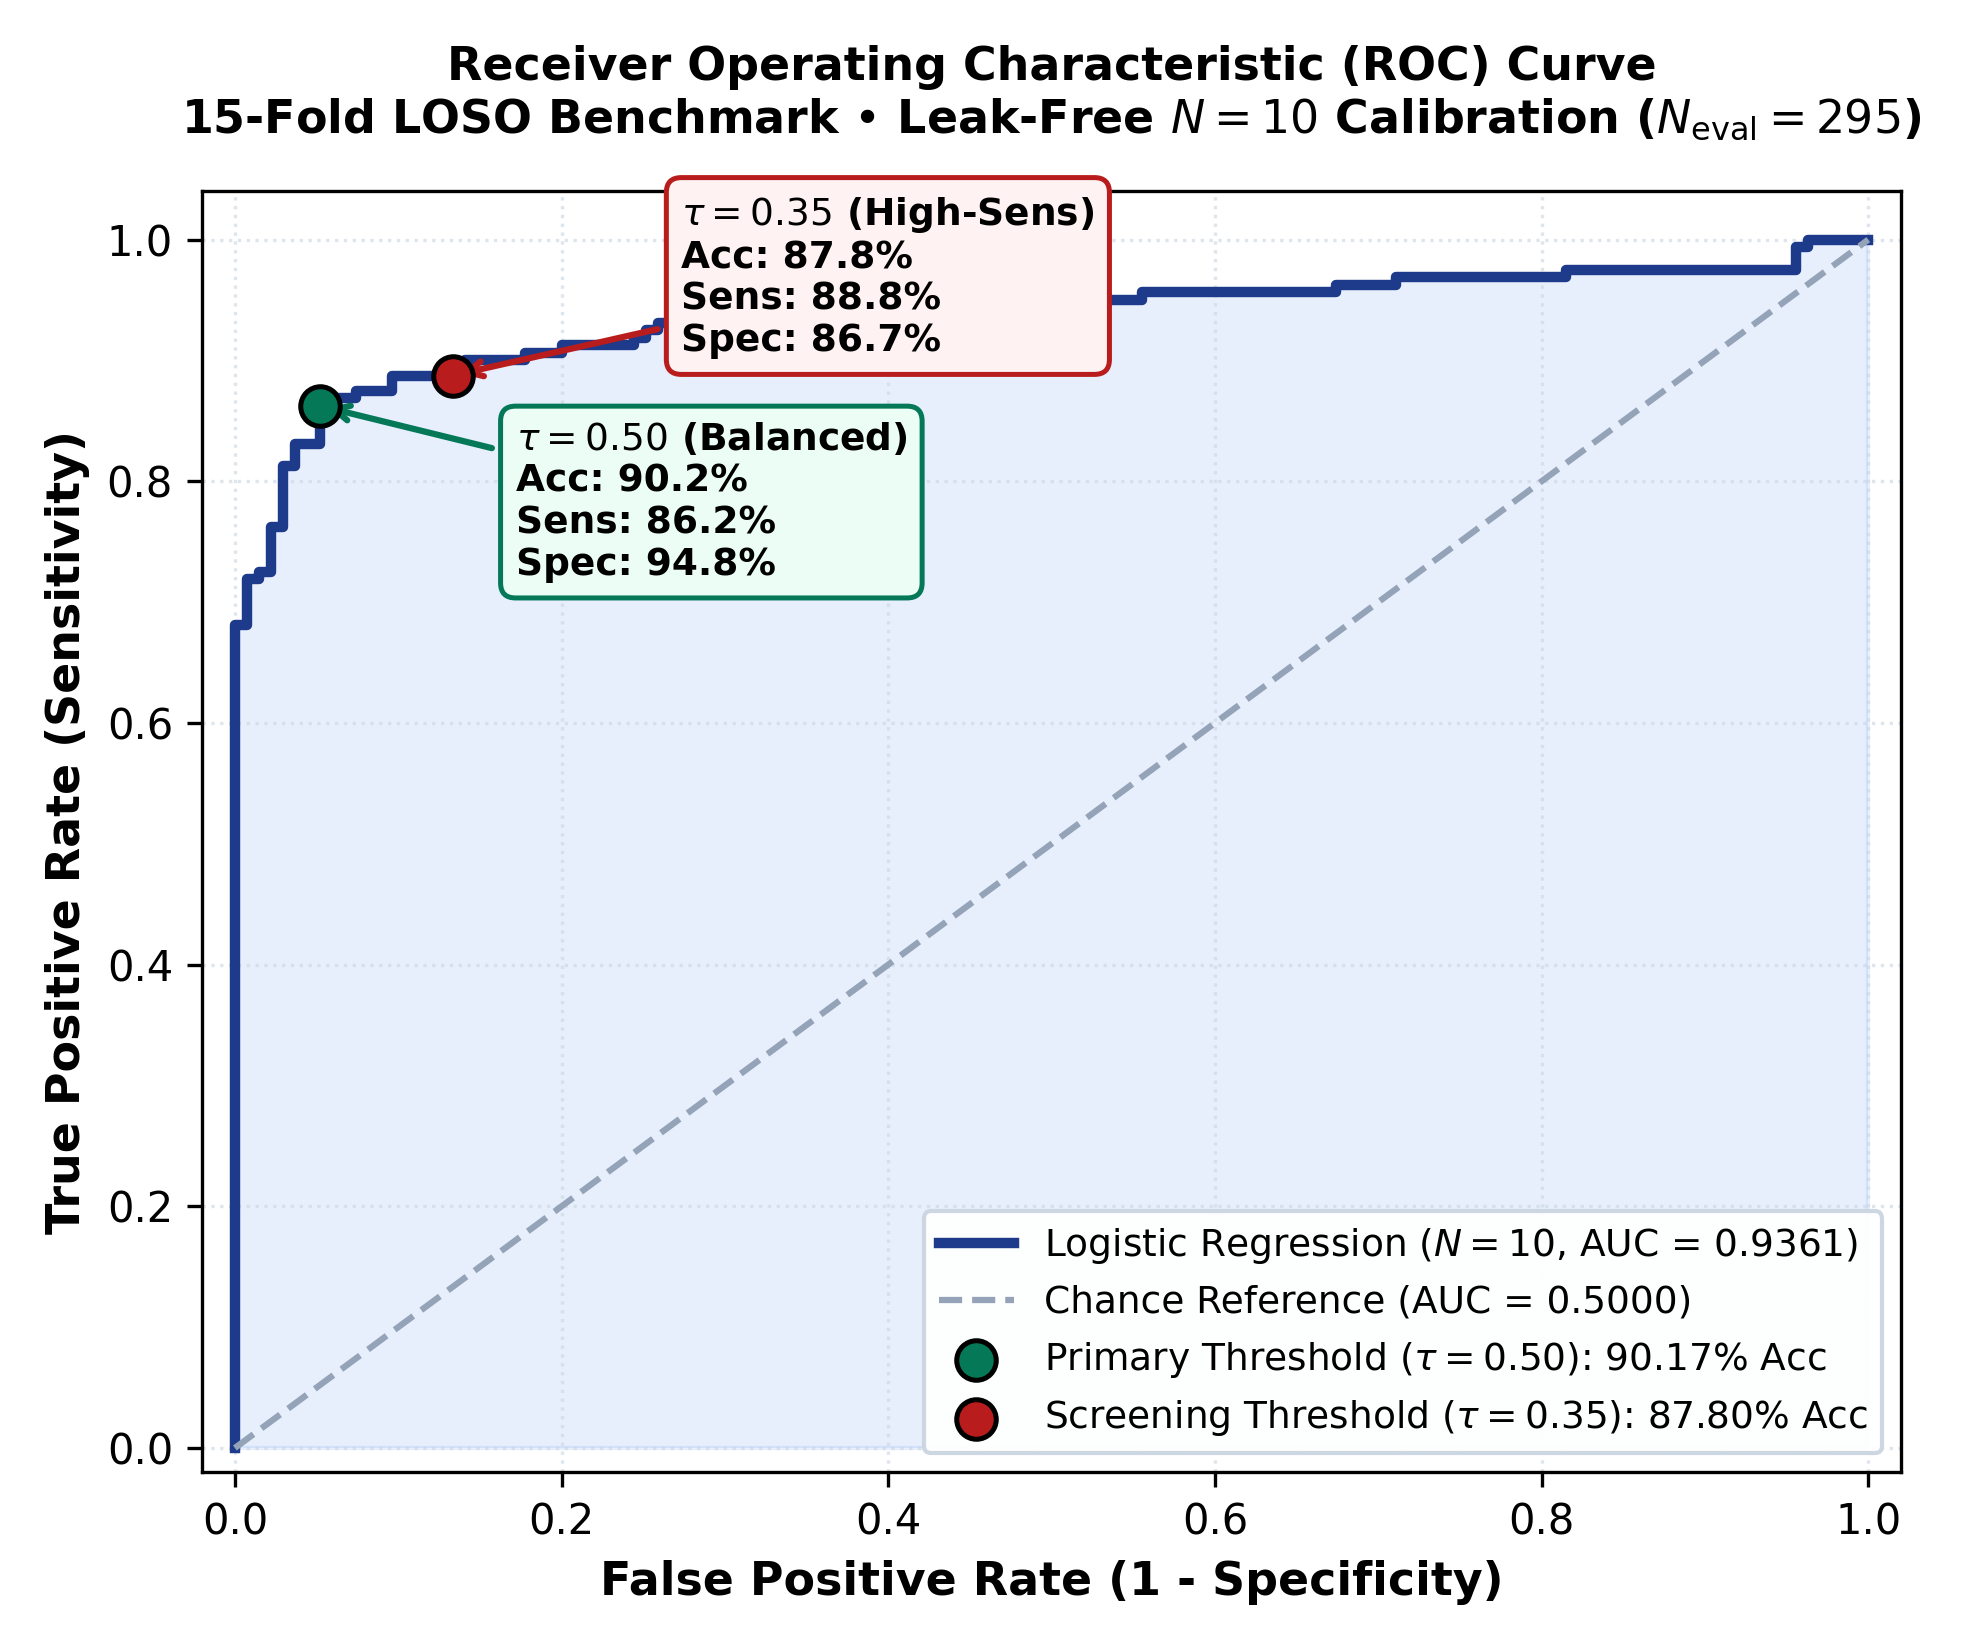
\includegraphics[width=\linewidth]{figures/FINAL_ROC_Curve.png}
    \caption{Receiver Operating Characteristic (ROC) curve under 15-fold LOSO cross-validation ($\text{ROC-AUC} = \valNtenRocAuc$) showing the primary operating point ($\tau = 0.50$) and screening threshold ($\tau = 0.35$).}
    \label{fig:roc_curve}
\end{figure}

\begin{figure}[t]
    \centering
    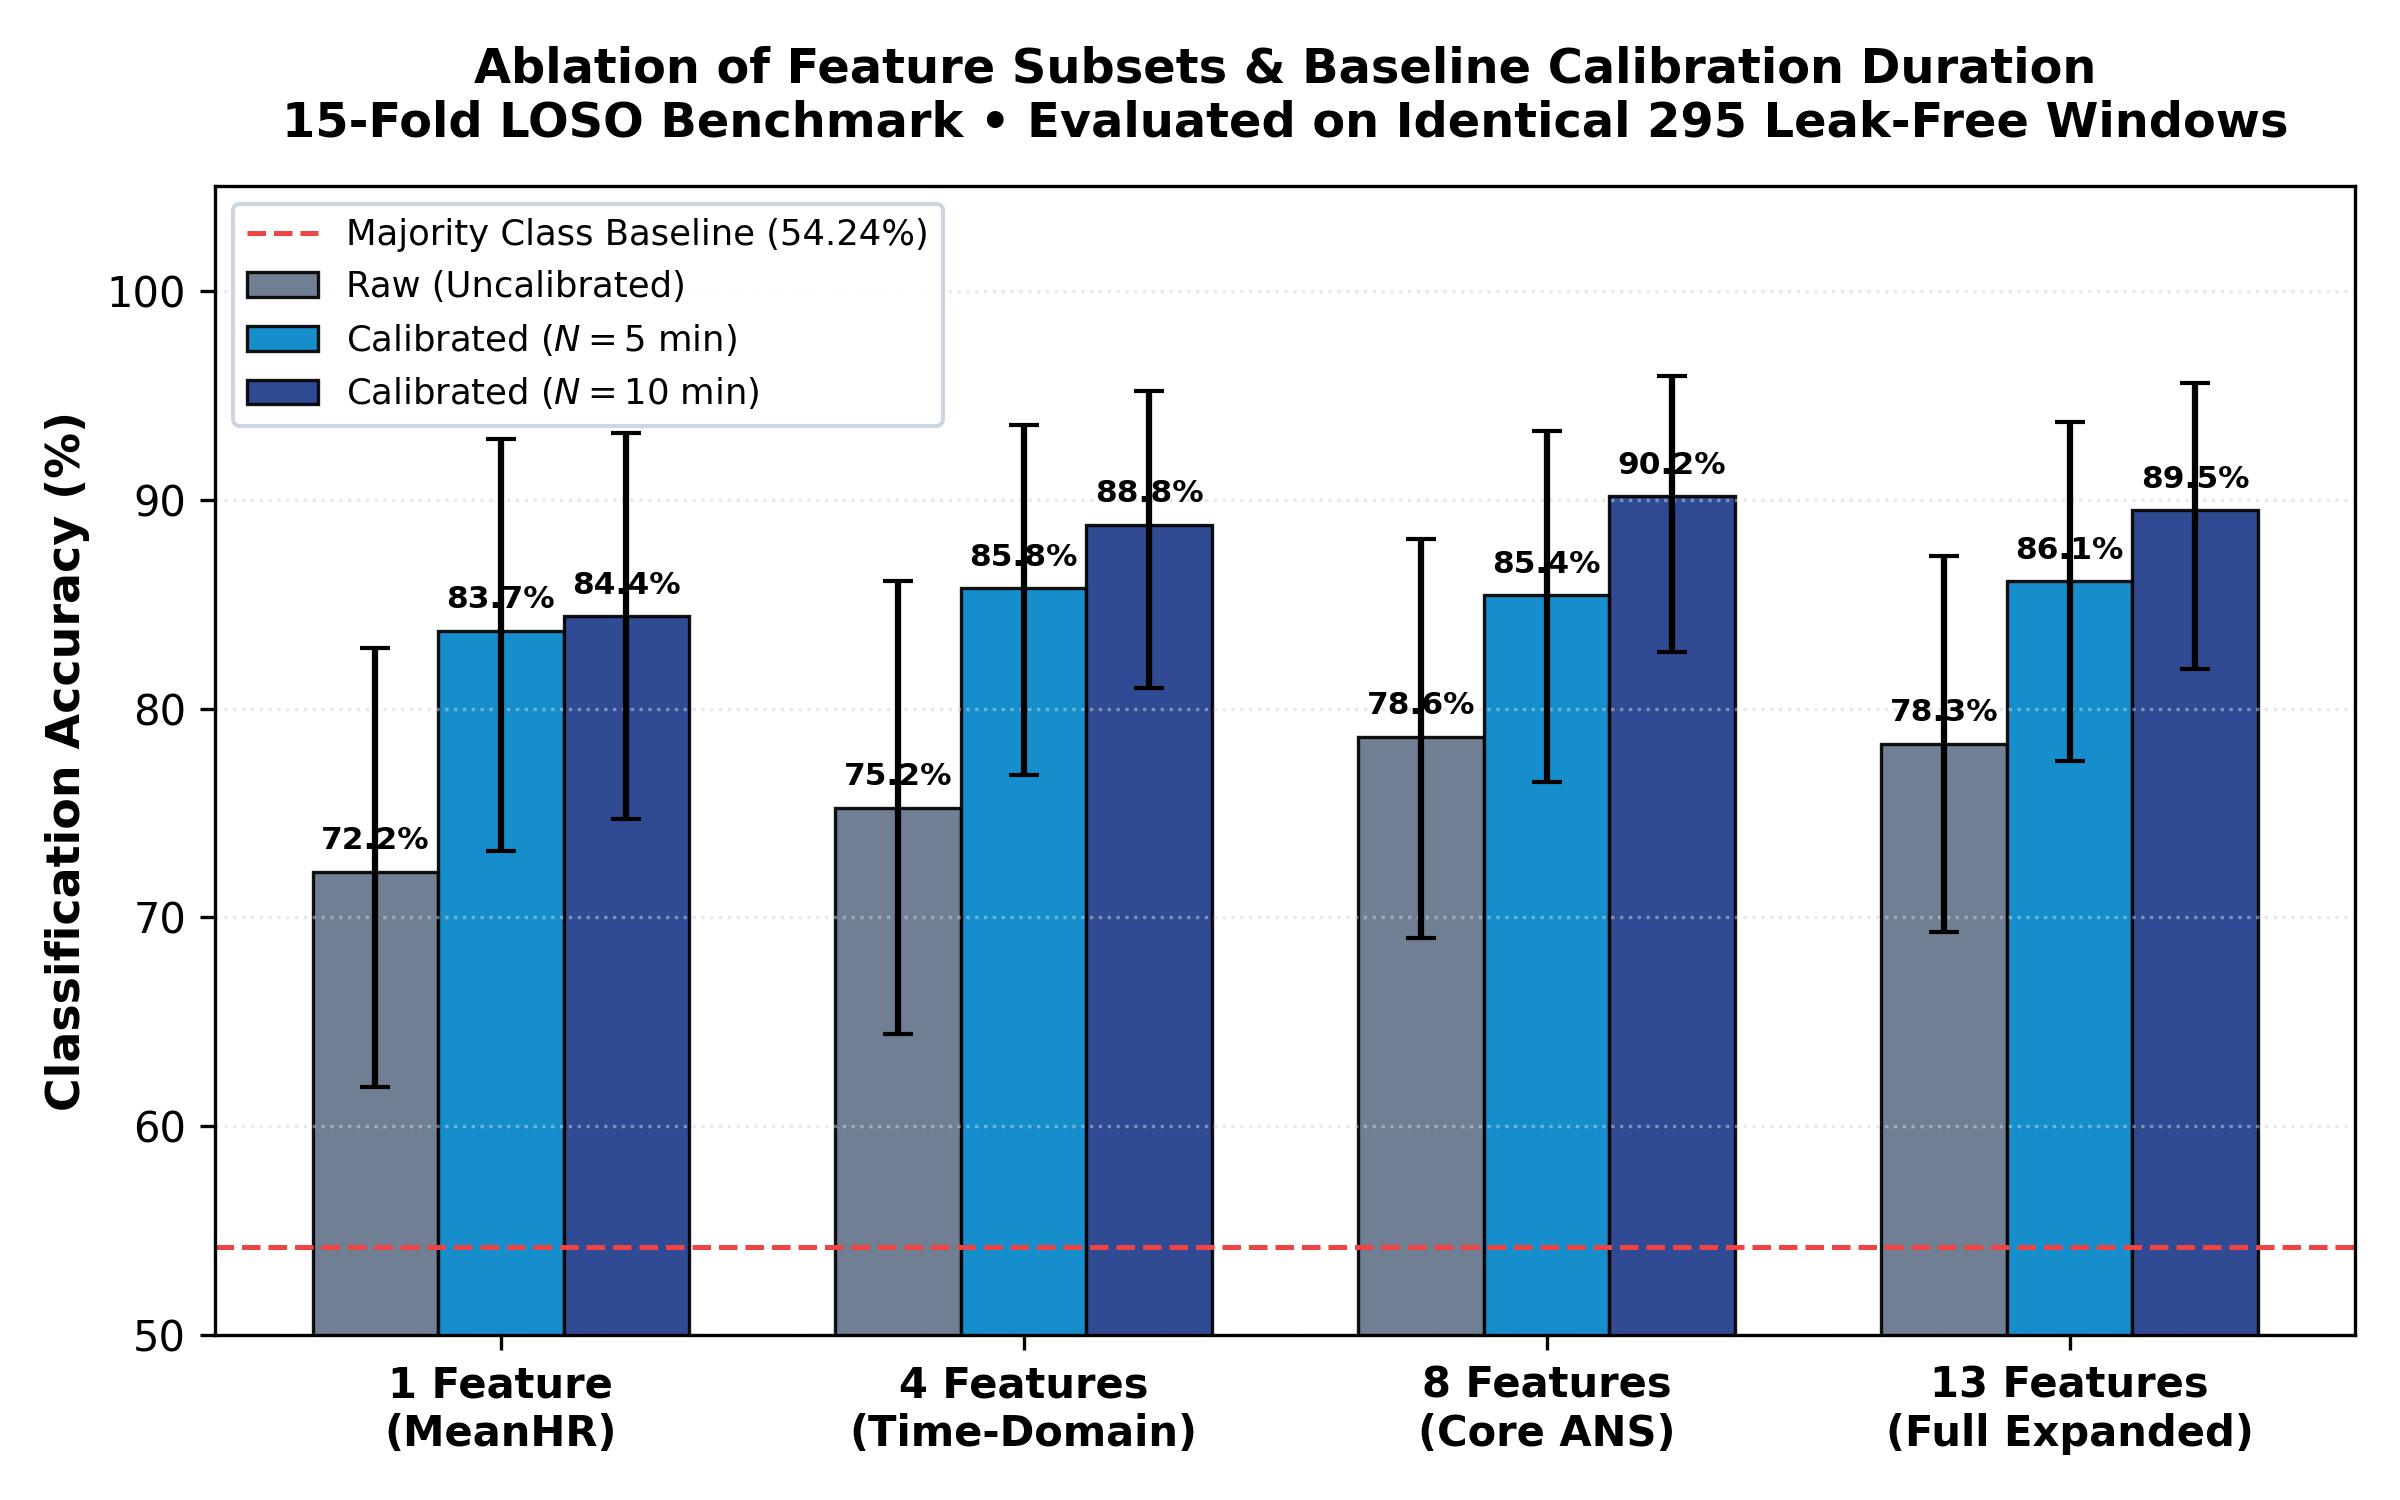
\includegraphics[width=\linewidth]{figures/FINAL_Personalized_Feature_Ablation.png}
    \caption{Ablation of feature subsets (1, 4, 8, 13 features) across Raw (uncalibrated), $N=5$, and $N=10$ baseline calibration on the \valEvalWindows common evaluation windows, with 95\% bootstrap confidence intervals.}
    \label{fig:ablation}
\end{figure}

\subsection{Calibration Duration and Paired Bootstrap Contrasts}
To determine the minimum resting calibration period necessary, we evaluated $N \in \{1, 2, 3, 5, 10\}$ chronological baseline windows on the identical \valEvalWindows evaluation windows using Logistic Regression. The full calibration duration curve is given in Table~\ref{tab:calibration_length}. 10,000-resample subject-level paired cluster bootstrap contrasts against uncalibrated Control (a) (\valControlNoCalibAccPct Acc, \valControlNoCalibBalAcc\% Bal Acc) are:
\begin{itemize}
    \item $N=1$: Acc $= \valNoneAcc\%$ [95\% CI: \valNoneAccCILow\%, \valNoneAccCIHigh\%], $\Delta\text{Acc} = \valPairedGainNone\text{ pp}$ [95\% CI: \valPairedGainNoneCILow, \valPairedGainNoneCIHigh] (crosses zero).
    \item $N=2$: Acc $= \valNtwoAcc\%$ [95\% CI: \valNtwoAccCILow\%, \valNtwoAccCIHigh\%], $\Delta\text{Acc} = \valPairedGainNtwo\text{ pp}$ [95\% CI: \valPairedGainNtwoCILow, \valPairedGainNtwoCIHigh] (crosses zero).
    \item $N=3$: Acc $= \valNthreeAcc\%$ [95\% CI: \valNthreeAccCILow\%, \valNthreeAccCIHigh\%], $\Delta\text{Acc} = \valPairedGainNthree\text{ pp}$ [95\% CI: \valPairedGainNthreeCILow, \valPairedGainNthreeCIHigh] (crosses zero).
    \item $N=5$: Acc $= \valNfiveAcc\%$ [95\% CI: \valNfiveAccCILow\%, \valNfiveAccCIHigh\%], $\Delta\text{Acc} = \valPairedGainNfive\text{ pp}$ [95\% CI: \valPairedGainNfiveCILow, \valPairedGainNfiveCIHigh] (interval excludes zero (unadjusted)).
    \item $N=10$ (selected post hoc as the best of the five lengths tested): Acc $= \valNtenAcc\%$ [95\% CI: \valNtenAccCILow\%, \valNtenAccCIHigh\%], $\Delta\text{Acc} = \valPairedGainNten\text{ pp}$ [95\% CI: \valPairedGainNtenCILow, \valPairedGainNtenCIHigh] (interval excludes zero (unadjusted)).
    \item $N=10$ minus $N=5$: $\Delta\text{Acc} = \valPairedGainNtenVsNfive\text{ pp}$ [95\% CI: \valPairedGainNtenVsNfiveCILow, \valPairedGainNtenVsNfiveCIHigh] (interval excludes zero (unadjusted)).
    \item $N=10$ minus Legacy Anchor (same \valEvalWindows\ windows, \valControlLeakyTwoNineFiveAccPct Acc): $\Delta\text{Acc} = \valPairedGainNtenVsLeaky\text{ pp}$ [95\% CI: \valPairedGainNtenVsLeakyCILow, \valPairedGainNtenVsLeakyCIHigh], showing no detectable difference. The legacy anchor evaluated across all \valTotalWindows windows achieved \valLegacyFourFourFiveAccPct accuracy \valLegacyFourFourFiveAccCI.
\end{itemize}

On the \valEvalWindows-window evaluation set, the legacy leaky anchor yields \valControlLeakyTwoNineFiveAccPct compared to \valNtenAccPct for $N=10$, showing no detectable difference on the 295-window set (\valPairedGainNtenVsLeaky~pp [95\% CI: \valPairedGainNtenVsLeakyCILow, \valPairedGainNtenVsLeakyCIHigh]); so the gain is attributable to calibrating at all, not to the earlier leaky anchor. Across the \valSubjTotalCount individual subjects, \valSubjImproveCount of \valSubjTotalCount improved, \valSubjUnchangedCount unchanged, \valSubjDecreaseCount worsened by at most one window.

\begin{table}[t]
\centering
\caption{Impact of Baseline Calibration Length on Leak-Free Evaluation ($N_{\text{eval}}=295$ Common Windows, 15 Subjects, $\tau = 0.50$)}
\label{tab:calibration_length}
{\footnotesize
\setlength{\tabcolsep}{2.5pt}
% Table: Calibration Length Evaluation (N_eval=295 common windows, tau=0.50)
\begin{tabular}{@{}lccccc@{}}
\toprule
\textbf{Config.} & \textbf{Acc [95\% CI]} & \textbf{B.Acc} & \textbf{F1} & \textbf{Sens} & \textbf{Spec} \\
\midrule
$N=1$ Min.  & 84.07 [75.2, 92.0] & 84.56 & 84.28 & 78.75 & 90.37 \\
$N=2$ Min.  & 83.39 [73.8, 91.8] & 83.99 & 83.39 & 76.88 & 91.11 \\
$N=3$ Min.  & 82.37 [73.0, 91.0] & 82.94 & 82.43 & 76.25 & 89.63 \\
$N=5$ Min.  & 85.42 [76.5, 93.3] & 86.10 & 85.32 & 78.12 & 94.07 \\
\textbf{$N=10$ Min.} & \textbf{90.17 [82.7, 95.9]} & \textbf{90.53} & \textbf{90.49} & \textbf{86.25} & \textbf{94.81} \\
\midrule
Ctrl (a): No Calib (295)  & 78.64 [69.0, 88.0] & 79.50 & 77.89 & 69.38 & 89.63 \\
Ctrl (b): Leaky (295)     & 89.83 [81.1, 96.7] & 90.51 & 89.80 & 82.50 & 98.52 \\
Legacy: Leaky (445)       & 92.13 [86.4, 97.1] & 90.02 & 88.29 & 82.50 & 97.54 \\
\bottomrule
\end{tabular}

}
\end{table}

\subsection{Leak-Free Feature Ablation}
Table~\ref{tab:ablation} details the multi-stage ablation across 4-feature, 8-feature, and 13-feature representations on the \valEvalWindows evaluation windows using Logistic Regression. Incorporating baseline calibration consistently elevates performance across all feature dimensions: 4 time-domain features improve from \valAblFourRawAcc\% to \valAblFourNtenAcc\%, and the core 8-feature set improves from \valAblEightRawAcc\% to \valNtenAccPct. Thirteen features did not improve on eight (\valAblThirteenNtenAcc\% vs \valNtenAccPct; intervals overlap), and the feature set was chosen post hoc.

\begin{table}[t]
\centering
\caption{Leak-Free Feature Ablation on Common \valEvalWindows\ Windows ($N=10$ Calibration, $\tau = 0.50$)}
\label{tab:ablation}
{\footnotesize
\setlength{\tabcolsep}{4pt}
% Table: Leak-Free Feature Ablation (Common 295 Windows, N=10 Calibration, tau=0.50)
\begin{tabular}{@{}llcc@{}}
\toprule
\textbf{M.} & \textbf{Feature Representation} & \textbf{Acc [95\% CI]} & \textbf{B.Acc} \\
\midrule
M1 & 4 Raw Features                 & 75.25 [64.4, 86.1] & 76.44 \\
M2 & 4 Calibrated ($N=10$)           & 88.81 [81.0, 95.2] & 89.34 \\
M3 & 8 Raw Features                 & 78.64 [69.0, 88.1] & 79.50 \\
\textbf{M4} & \textbf{8 Calibrated (Prop. $N=10$)} & \textbf{90.17 [82.7, 95.9]} & \textbf{90.53} \\
M5 & 13 Raw Features                & 78.31 [69.3, 87.3] & 79.07 \\
M6 & 13 Calibrated ($N=10$)          & 89.49 [81.9, 95.6] & 89.85 \\
\midrule
\multicolumn{4}{@{}l}{\textit{Legacy Reference (All-Baseline Anchor, 445 Windows):}} \\
Ref & 8 Calibrated (Leaky, 445 win) & 92.13 [86.4, 97.1] & 90.02 \\
\bottomrule
\end{tabular}

}
\end{table}

\subsection{Decision Threshold Sensitivity}
Table~\ref{tab:thresholds} reports classification sensitivity across decision thresholds $\tau$. At the standard balanced threshold ($\tau = 0.50$), the model achieves \valNtenAccPct accuracy, \valNtenSensPct sensitivity, and \valNtenSpecPct specificity. Lowering the decision threshold to $\tau = 0.35$ raises sensitivity to \valTauThirtyFiveSensPct (specificity: \valTauThirtyFiveSpecPct, accuracy: \valTauThirtyFiveAccPct).

\begin{table}[t]
\centering
\caption{Decision Threshold Sensitivity Comparison on 295 Windows}
\label{tab:thresholds}
{\footnotesize
\setlength{\tabcolsep}{4pt}
% Table: Decision Threshold Sensitivity Comparison
\begin{tabular}{@{}lcccc@{}}
\toprule
\textbf{Protocol} & \textbf{Threshold} & \textbf{Acc} & \textbf{Sens} & \textbf{Spec} \\
\midrule
$N=10$ (295 win) & $\tau = 0.50$ (Std.)  & 90.17 & 86.25 & 94.81 \\
$N=10$ (295 win) & $\tau = 0.35$ (Screen) & 87.80 & 88.75 & 86.67 \\
\midrule
Ctrl (b): Leaky (295) & $\tau = 0.50$ & 89.83 & 82.50 & 98.52 \\
Legacy Ref: Leaky (445) & $\tau = 0.50$ & 92.13 & 82.50 & 97.54 \\
Legacy Ref: Leaky (445) & $\tau = 0.35$ & 92.36 & 86.25 & 95.79 \\
\bottomrule
\end{tabular}

}
\end{table}

\section{Embedded Microcontroller Execution and Telemetry Replay}

To evaluate embedded feasibility, the biquad filter and the telemetry framing were implemented and tested with replayed WESAD samples; no live ECG sensor was connected. The \valFlashSampleCount flash samples were downsampled to 350~Hz from Subject S2 (representing \valFlashSampleSec seconds) and replayed at 350~Hz via SysTick timer interrupts over USART2 at \valUartBaudRate baud. The embedded filter is a causal 5-stage Direct Form I biquad cascade (four 2nd-order stages implementing a 4th-order Butterworth 0.5--40~Hz bandpass and one 2nd-order 50~Hz notch) running sample-by-sample at 350~Hz; the offline experiments use a zero-phase 4th-order Butterworth bandpass filter (0.5--40~Hz) with \texttt{filtfilt} at \valSamplingRateHz~Hz. Classification accuracy was not evaluated with the embedded filter; baseline calibration and Logistic Regression run on the host.

\subsection{Digital Filter Hardware Execution Benchmarking}
Hardware execution latency was measured directly on physical silicon across \valDwtTrialCount independent single-sample filter trials using the internal ARM Cortex-M Data Watchpoint and Trace (DWT) cycle counter (\texttt{DWT->CYCCNT}). The empirical distribution recorded:
\begin{itemize}
    \item Minimum Execution: \valBiquadMinCycles cycles (\valBiquadMinUs~$\mu\text{s}$)
    \item Mean Execution: \valBiquadMeanCycles cycles (\valBiquadMeanUs~$\mu\text{s}$)
    \item Maximum Execution: \valBiquadMaxCycles cycles (\valBiquadMaxUs~$\mu\text{s}$)
\end{itemize}

At a 350~Hz cardiac sampling rate, continuous single-sample filtering consumes:
\begin{equation}
\begin{aligned}
    \text{CPU Utilization} &= \frac{\valBiquadMeanCycles \text{ cycles/sample} \times 350 \text{ Hz}}{170 \times 10^6 \text{ Hz}} \times 100\% \\
    &= \valBiquadCpuLoad
\end{aligned}
\end{equation}
leaving $>99.9\%$ of processor cycles available for other tasks.

\begin{figure}[t]
    \centering
    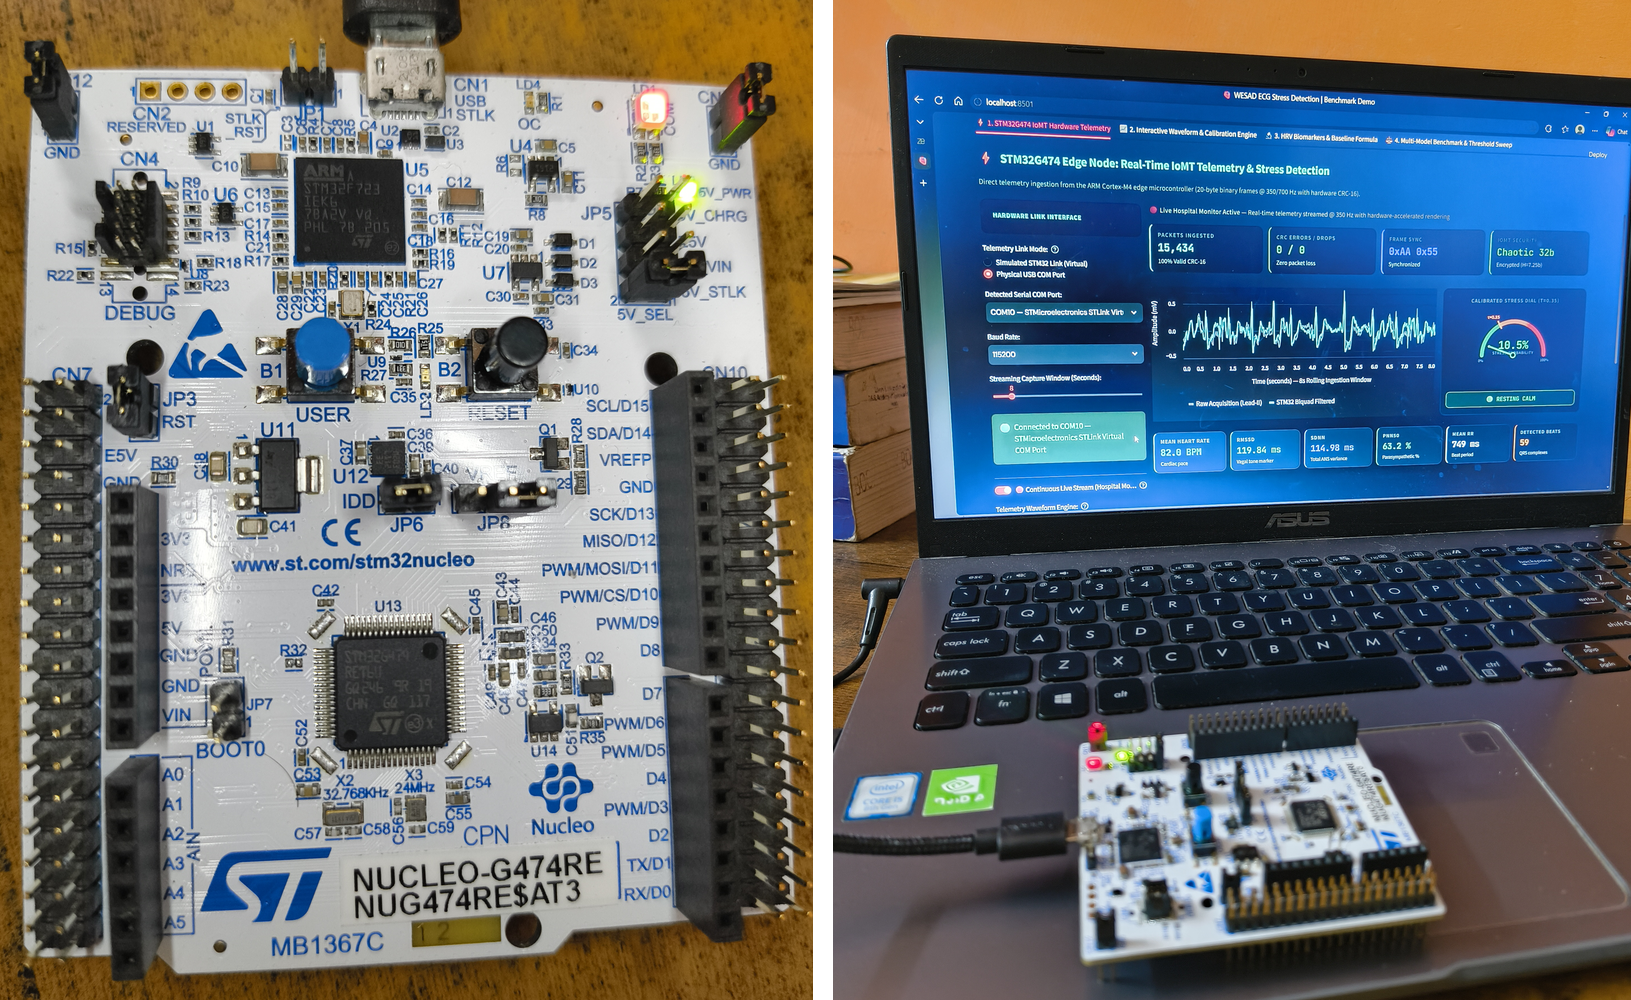
\includegraphics[width=\linewidth]{figures/FIG_Hardware_Testbed_Composite.png}
    \caption{Bare-metal ARM Cortex-M4 (STM32G474RE) hardware testbed: (a) Nucleo-G474RE development board; (b) host running the dashboard visualizer.}
    \label{fig:hw_testbed}
\end{figure}

\begin{table}[t]
\centering
\caption{Hardware-in-the-Loop Telemetry and Resource Profile}
\label{tab:hw_profile}
{\footnotesize
\setlength{\tabcolsep}{2pt}
% Table: Hardware-in-the-Loop Telemetry and Resource Profile
\begin{tabular}{@{}lll@{}}
\toprule
\textbf{Metric} & \textbf{Value / Measurement} & \textbf{Specification} \\
\midrule
MCU Platform         & STM32G474RE (Cortex-M4) & 170~MHz, FPU \\
Biquad Latency       & \valBiquadMeanUs~$\mu\text{s}$ (\valBiquadMeanCycles cycles) & \valBiquadCpuLoad load \\
UART Baud Rate       & \valUartBaudRate baud (350.02 Hz)& 20-byte wire frame \\
HIL Source           & WESAD S2 Baseline in Flash & \valFlashSampleCount samples \\
HIL Packet Count     & \valHilPackets consecutive pkts & \valHilWireBytes wire bytes \\
Packet Loss Rate     & 0.00\% (0 lost packets) & Strict 16-bit CRC \\
Plaintext Recovery   & 100.00\% exact recovery & Zero bit errors \\
Payload Entropy      & $H = \valWireEntropy$~bits/byte  & Bytes 10..17 (\valHilPayloadBytes B) \\
Payload Uniformity   & $\chi^2 = \valChiSquareStat$ ($p=\valChiSquareP$) & No rejection ($\alpha=0.01$) \\
\bottomrule
\end{tabular}

}
\end{table}

\subsection{Lightweight Telemetry Obfuscation Layer}
To provide physical-layer data masking against casual passive eavesdropping on wireless links without cryptographic key management overhead, we implemented a 4-dimensional coupled hyperchaotic keystream generator (HC1):
\begin{equation}
\begin{aligned}
\dot{x} &= a(y - x) + w \\
\dot{y} &= cx - xz + dy \\
\dot{z} &= xy - bz \\
\dot{w} &= -rx
\end{aligned}
\label{eq:hc1_ode}
\end{equation}
with system parameters $a=15.81, b=2.76, c=86.03, d=-9.07, r=10.79$, numerically estimated Lyapunov exponents $\lambda_1 = \valLyapunovPrimaryLOne$ and $\lambda_2 = \valLyapunovPrimaryLTwo$ (ranges across step sizes, integration durations and initial conditions: $[\valLyapunovRangeLOneLow, \valLyapunovRangeLOneHigh]$ and $[\valLyapunovRangeLTwoLow, \valLyapunovRangeLTwoHigh]$), with a Kaplan--Yorke dimension of $D_{KY} = \valLyapunovPrimaryDKY$. The phase-space divergence is constant everywhere:
\begin{equation}
    \nabla \cdot \mathbf{F} = \operatorname{Tr}(J) = -a + d - b = \valDivergence
\end{equation}
confirming strictly dissipative dynamics.

\subsection{Hardware-in-the-Loop Replay Validation}
As summarized in Table~\ref{tab:hw_profile}, to evaluate telemetry link reliability, \valHilPackets consecutive 20-byte binary packets (\valHilWireBytes bytes total on wire, \valHilPayloadBytes scrambled payload bytes) were streamed over physical USART2 at \valUartBaudRate baud. Bit-exact plaintext recovery was verified across all \valHilPackets packets with zero CRC errors and zero packet loss. Shannon entropy $H = \valWireEntropy$ bits/byte and Chi-square $\chi^2 = \valChiSquareStat$ ($p = \valChiSquareP, \text{df} = 255$) were computed on the \valHilPayloadBytes scrambled payload bytes (bytes 10..17), showing no rejection of uniformity at $\alpha = 0.01$; full-frame entropy is \valFullFrameEntropy bits/byte because of static headers. We did not run the NIST suite. Fig.~\ref{fig:dashboard} demonstrates the replayed host monitoring interface.

\begin{figure}[t]
    \centering
    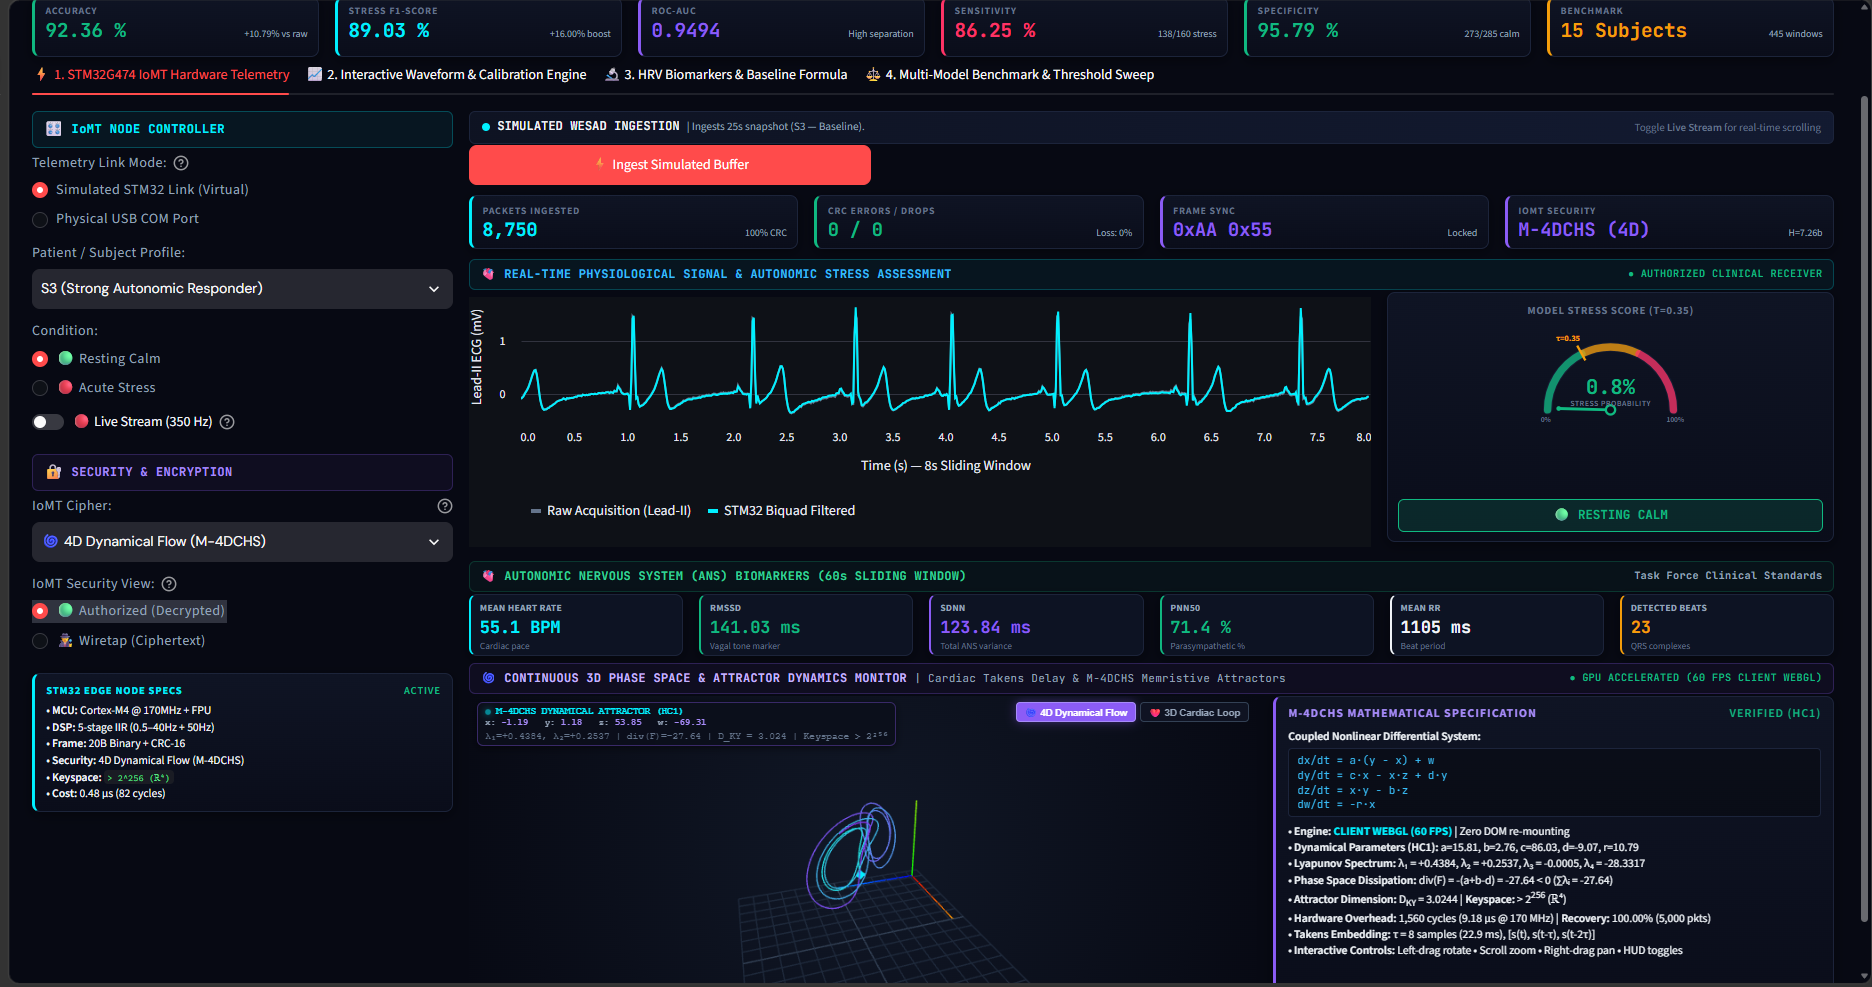
\includegraphics[width=\linewidth]{figures/FIG_Dashboard_SinglePage_M4D_Descrambled.png}
    \caption{Demonstration of the host monitoring interface replaying single-channel chest ECG (RespiBAN, \valSamplingRateHz~Hz) telemetry: descrambled ECG stream, stress probability index, beat-to-beat HRV indices, and synchronized live visualizer (demonstration fitted across the full session).}
    \label{fig:dashboard}
\end{figure}

\section{Limitations}
\label{sec:limitations}
Several methodological and clinical considerations bound our findings:
\begin{enumerate}
    \item Post hoc selection of the 8-feature representation, decision thresholds ($\tau=0.50$ and $\tau=0.35$), and the $N=10$ minute calibration window duration on the same 15 WESAD subjects; reported confidence intervals are unadjusted for multiple contrasts and post hoc selection.
    \item Calibration gains at $N \le 3$ were not detectable with 15 subjects, which does not show short calibration is useless, and larger cohorts may be needed to measure small effects.
    \item One recording session per person without multi-day longitudinal tracking, evaluated on a young, healthy laboratory cohort ($27.5 \pm 2.4$ years) without cardiovascular pathology or uncontrolled ambulatory movement.
    \item Binary baseline-vs-stress classification task, with other emotional states (amusement, meditation) excluded.
    \item \valWindowDurationSec-second analysis windows limit spectral estimation resolution, particularly in the Low-Frequency (LF: 0.04--0.15~Hz) band, compared with the 5-minute standard recommended by clinical guidelines \cite{taskforce1996hrv}.
    \item Baseline calibration requires windows known to represent resting state, which a deployed ambulatory system must be capable of automatically identifying.
    \item The embedded filter (causal 5-stage biquad cascade at 350~Hz) differs from the offline preprocessing pipeline (zero-phase Butterworth at \valSamplingRateHz~Hz), and classification accuracy was not evaluated with the embedded filter; the HIL test replays stored samples, and baseline calibration and Logistic Regression inference run on the host.
    \item The HC1 hyperchaotic keystream engine provides physical-layer obfuscation without key management or formal cryptanalysis; it is not a replacement for standard authenticated cryptography.
\end{enumerate}

\section{Conclusion}
This study investigated the impact of baseline calibration duration for acute psychological stress detection from single-channel chest ECG under a leak-free evaluation protocol. By anchoring normalization on the first $N$ chronological resting baseline windows and excluding calibration windows from test scoring, 15-fold Leave-One-Subject-Out cross-validation on the common \valEvalWindows-window evaluation set demonstrated that $N=10$ achieves \valNtenAccPct accuracy [95\% CI: \valNtenAccCILow\%, \valNtenAccCIHigh\%] and \valNtenFOnePct F1-score [95\% CI: \valNtenFOneCILow\%, \valNtenFOneCIHigh\%], representing a paired gain whose interval excludes zero of \valPairedGainNten percentage points over uncalibrated features. The interval also excludes zero at $N=5$ (\valPairedGainNfive pp), whereas calibrations at $N \le 3$ minutes yielded confidence intervals crossing zero. The choice of $N = 10$ and the feature set were selected post hoc. Embedded execution on an ARM Cortex-M4 microcontroller demonstrated a per-sample cost of \valBiquadMeanUs~$\mu\text{s}$ (\valBiquadMeanCycles cycles) for Biquad filtering and a \valHilPackets-packet HIL replay with exact payload recovery and no CRC errors.

Code, results and the build are in the public repository \url{https://github.com/Mukesh-Yadav-4/ECG_STRESS_DETECTION}; an archived release DOI will be added.

\section*{Acknowledgment}
AI tools (Antigravity, ChatGPT, Claude) were used for code development and for editing and cross-checking text. The author reviewed all outputs and takes full responsibility for the content.

\bibliographystyle{IEEEtran}
\bibliography{refs}

\end{document}
